\documentclass[a4paper,12pt]{scrartcl}
\usepackage[utf8]{inputenc}
\usepackage[UKenglish]{isodate}
\usepackage{csquotes}
\usepackage{graphicx}
\usepackage{wrapfig}
\usepackage{enumitem}
\usepackage{pdflscape}
\usepackage[toc,page]{appendix}
\usepackage{geometry}
\usepackage{hyperref}
\usepackage{cleveref}
\usepackage{listings}
\usepackage{csvsimple}
\usepackage{booktabs}
\usepackage{longtable}
\usepackage{caption}
\usepackage{subcaption}
\usepackage[colorinlistoftodos]{todonotes}
\usepackage[british]{babel}
\usepackage{float}
%\usepackage[margin=1in]{geometry}
\usepackage{listings}
\usepackage{color}
 
\definecolor{codegreen}{rgb}{0,0.6,0}
\definecolor{codegray}{rgb}{0.5,0.5,0.5}
\definecolor{codepurple}{rgb}{0.58,0,0.82}
\definecolor{backcolour}{rgb}{0.95,0.95,0.92}
 
\lstdefinestyle{mystyle}{
	language=PHP,
    backgroundcolor=\color{backcolour},   
    commentstyle=\color{codegray},
    keywordstyle=\color{magenta},
    numberstyle=\tiny\color{codegray},
    stringstyle=\color{codegreen},
    basicstyle=\footnotesize,
    breakatwhitespace=false,         
    breaklines=true,                 
    captionpos=b,                    
    keepspaces=true,                 
    numbers=left,                    
    numbersep=5pt,                  
    showspaces=false,                
    showstringspaces=false,
    showtabs=false,                  
    tabsize=3,
    morekeywords={ new, __halt_compiler, abstract, and, array, as, break, callable, case, catch, class, clone, const, continue, declare, default, die, do, echo, else, elseif, empty, enddeclare, endfor, endforeach, endif, endswitch, endwhile, eval, exit, extends, final, for, foreach, function, global, goto, if, implements, include, include_once, instanceof, insteadof, interface, isset, list, namespace, new, or, print, private, protected, public, require, require_once, return, static, switch, throw, trait, try, unset, use, var, while, xor}
}

\lstset{language=Java,
  showspaces=false,
  showtabs=false,
  breaklines=true,
  showstringspaces=false,
  breakatwhitespace=true,
  commentstyle=\color{pgreen},
  keywordstyle=\color{pblue},
  stringstyle=\color{pred},
  basicstyle=\ttfamily,
  moredelim=[il][\textcolor{pgrey}]{$$},
  moredelim=[is][\textcolor{pgrey}]{\%\%}{\%\%}
}
 
\lstset{style=mystyle}

\graphicspath{ {images/} }
\usepackage[
	backend=biber,
	style=ieee,
	]{biblatex}

\addbibresource{references.bib}

\title{829H1 Real-Time Embedded Systems Exercise 4}
\author{Candidate No: 105936}
\date{\today}

\begin{document}
	
	\begin{titlepage}
		\maketitle
	\end{titlepage}
	
	\tableofcontents
	\newpage
	
	\section{Introduction}
	{
		This report focuses on using serial communications on the board and shows the work completed during the laboratory sessions, what equipment was used and what was learnt. Code listings for some of the created programs can be found in \cref{Appendix:start}.
	}

	\section{Equipment}
	{
		\subsection{Hardware}{
			The experiments carried out in this report were run on the Freedom-K64F prototyping board\cite{nxpproducts2014}. To use this board, we needed to connect the board to the computer using the debug port and copy across the program we wish to run and then press the reset button to load the program.
			\begin{figure}[h]
				\centering
				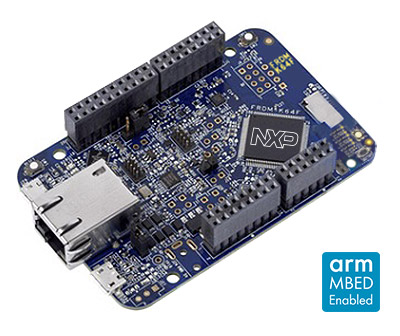
\includegraphics[width=0.5\textwidth]{FRDM-K64F-ANGLE}
				\caption{An Image of the Freedom-K64F Board used during experimentation\cite{nxpproducts2014}}
				\label{img:FRDM-K64F}
			\end{figure}
			We also needed to use an oscilloscope in the exercise, for this you usually need to know what pin you are outputting to, therefore I used \cref{img:pinout} to find this.
			\begin{figure}[h]
				\centering
				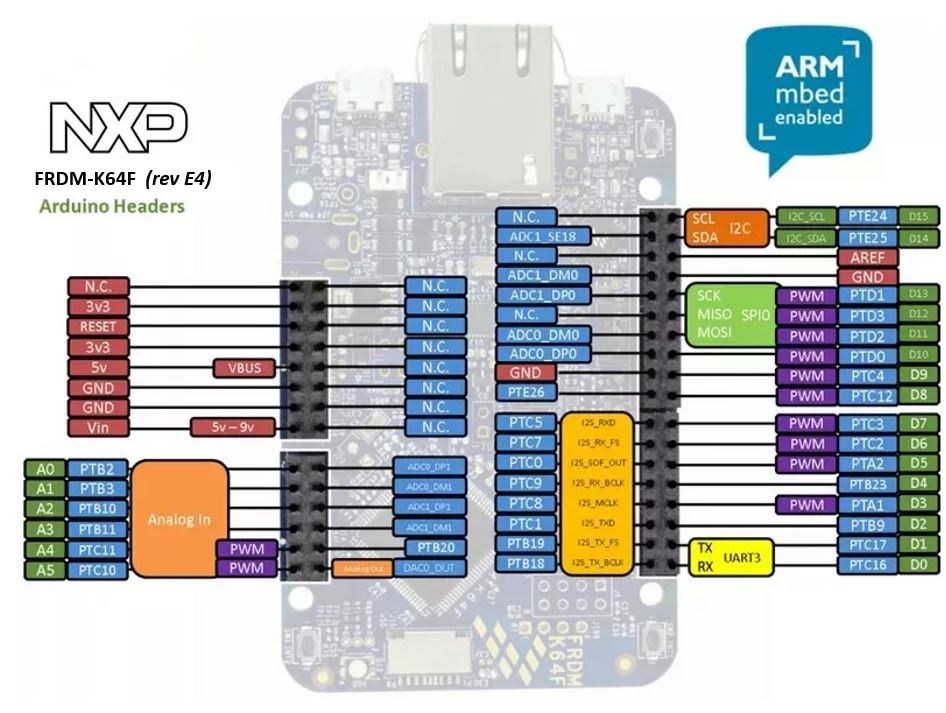
\includegraphics[width=0.5\textwidth]{frdm_k64f_reve4_header_pinout}
				\caption{An Image showing the pin names one the Freedom-K64F Board\cite{armlimited2015}}
				\label{img:pinout}
			\end{figure}
		}
		\subsection{Software}
		{
			To develop the experiments, I used Arm's mbed cloud IDE. This allows users to write c++ code and compile it to a device of their choice. 
		}
	}
	
	\section{Experiments}
	{
		\subsection{Serial Communications}
		{
			For this experiment I created a SPI master object which allowed me to output data using serial methods on three pins, these pins were PTD2 which was the MOSI, PTD3 the MISO and PTD1 which was the clock.
			\subsubsection{Using Different SPI Modes}
			{
				This changes the clock signal
			}
		}
		\subsection{Linking Two Boards together}
		{

		}
	}

	\section{Conclusion}
	{
		In conclusion, this was a useful quick introduction into how to develop using interrupts and timers also learning how to use tera term to view the console output of the board.
	}
	
	\newpage
	\begin{appendices}
	\label{Appendix:start}
	\section{Lab Exercise 1}
	{
		\subsection{Part 1}
		{
			\label{appendix:ex1-1}
			\lstinputlisting[language=c++]{CodeListings/Ex1/mainPart1.cpp}
		}
		\subsection{Part 2}
		{
			\label{appendix:ex1-2}
			\lstinputlisting[language=c++]{CodeListings/Ex1/mainPart2.cpp}
		}
		\subsection{Part 3}
		{
			\label{appendix:ex1-3}
			\lstinputlisting[language=c++]{CodeListings/Ex1/mainPart3.cpp}
		}
	}
	\section{Lab Exercise 2}
	{
		\label{appendix:ex2}
		\subsection{Part 1 - Master Program}
		{
			\label{appendix:ex2-1}
			\lstinputlisting[language=c++]{CodeListings/Ex2/main-master.cpp}
		}
		\subsection{Part 2 - Slave Program}
		{
			\label{appendix:ex2-2}
			\lstinputlisting[language=c++]{CodeListings/Ex2/main-slave.cpp}
		}
	}

\end{appendices}
	\printbibliography[heading=bibintoc,title=References]
\end{document}
